\documentclass[conference]{IEEEtran}

% Write an eight page technical paper describing your project in the style of an IEEE Visualization Technical Paper (other formats may be acceptable with pre-approval).

% Sections you should plan to include are: abstract, introduction, related work (adapt your literature review for this), implementation, results, future directions, and references.

% Your paper should include figures and images as appropriate.

% A complete draft of your paper, including figures and images, must be submitted in advance of the final paper deadline.

% Your draft should be a complete paper that is as strong and polished as you can make it.

% Aim for something that you believe is ready for submission to a conference or journal.

% The course instructor will serve as reviewer for these papers and make suggestions as to how they might be improved.

% You may submit earlier, not necessarily complete, drafts of your paper if you would like feedback earlier in the writing process.

% Correct spelling and grammar count in all submitted work, so check them before you hand anything in.



\usepackage{epsfig}

% Example figure
%\begin{figure}[ht]
% \centering
% \includegraphics[scale=.8]{old.png}
% \caption{}
% \label{old}
% \end{figure}


\begin{document}

\title{SwarmVis: a Tool for Visualizing Swarm Systems}

\author{\IEEEauthorblockN{Don Miner}
\and
\IEEEauthorblockN{Niels Kasch}
}
\maketitle


\begin{abstract}
In this paper, we provide an overview of SwarmVis, a tool for visualizing swarm systems. SwarmVis is able to create informative still images and videos of swarm systems moving in two- and three- dimensional spaces through the use of several visualization techniques. We discuss what information about swarms needs to be conveyed and then explain in detail how we tackled these individually in SwarmVis. Finally, we use two case studies, a tetrahedron and a boid flock, to demonstrate how SwarmVis can be used to analyze both the low-level and swarm-level behaviors of a multi-agent system.


\end{abstract}

\section{Introduction}
Swarm systems are a group of agents that exhibit some collective behavior. Examples of these systems include: social animals (e.g. bees, ants, schooling fish, migrating geese), particles in liquids,  and multi-robot systems. Visualizing swarm systems (swarms) effectively is difficult due to the large number of individual agents contained. A typical swarm's high density and chaotic motions amplify the complexity of swarm visualization. Effective swarm visualizations are needed to provide insight into swarm behavior and inspect local interactions.
A well defined set of visualization techniques would provide researchers with these insights.

\begin{figure}[ht]
\centering
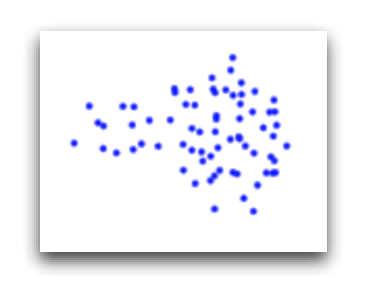
\includegraphics[scale=1]{images/basic.pdf}
\caption{A basic visualization of a swarm that only plots points in space. Note that important properties such as direction, velocity
and previous positions are not conveyed.}
\label{old}
\end{figure}

Crude visualization techniques plot the position of each agent in space as seen with a Reynolds boid flock\cite{reynolds1987} in Figure \ref{old}. A still image only shows the location of individual agents and does not convey important information such as the direction, velocity, and previous positions.
We have implemented \textit{SwarmVis}, a toolkit for visualizing swarms, that goes beyond the simple plotting technique to solve these problems. The toolkit aims to provide visualization techniques that allow researchers to interactively investigate swarms so that researchers will be able to study interactions, fine-grained movements, and swarm behavior. Figure \ref{ShowOff} displays a swarm system with
the addition of our trails visualization and conveys much more information than Figure \ref{old}.

\begin{figure}[ht]
\centering
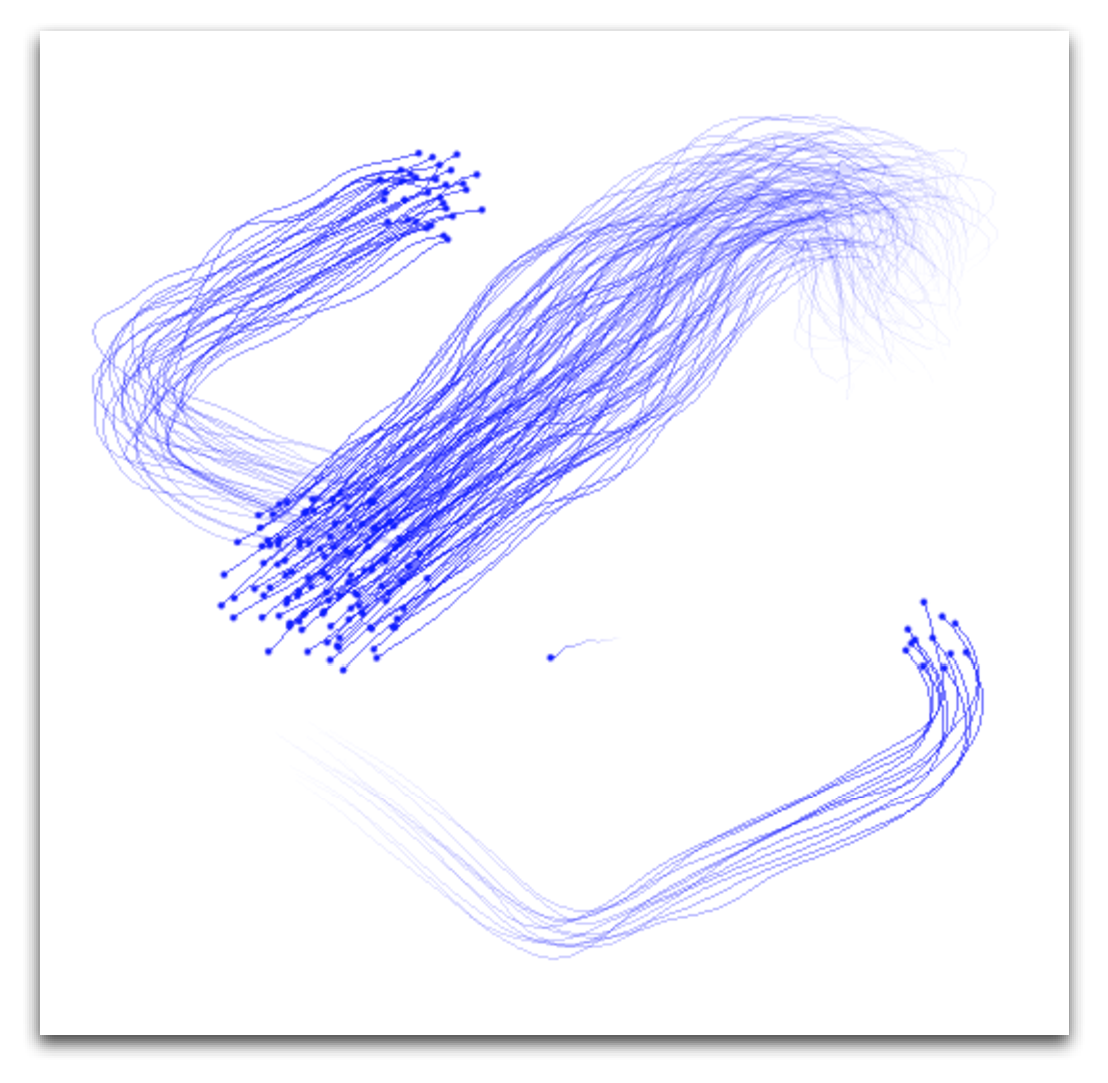
\includegraphics[scale=.42]{images/showoff.pdf}
\caption{A basic visualization of a swarm that only plots points in space as well as trails of significant length.
Note that important properties such as direction, velocity, structure, rotation,
and previous positions are conveyed.}
\label{ShowOff}
\end{figure}

The goal of SwarmVis is to facilitate, through visualization, the detailed analysis of emergent behavior that results from swarm systems. In order to satisfy this objective, we have created a software toolkit with the following high-level application goals and requirements in mind:
\begin{itemize}
\item The toolkit shall visualize swarms using a series of still images (i.e. a video) embedded in an interactive framework that has features such as pausing, slowing down and rewinding of frames.
\item Agent position, direction and velocity shall be conveyed through both still images and videos generated from the software.
\item The toolkit shall provide a variety of built-in visualization techniques that are useful in visualizing swarm systems.
\end{itemize}

In this paper, we discuss previous work in swarm system visualization,
some of which has provided inspirations for the techniques in SwarmVis.
Then, we discuss the implementation details of the user interface and graphical visualization.
We conclude with an overview of the projects and an analysis of its effectiveness.
A brief user guide for compiling, running and loading data in SwarmVis is provided in the appendix.

\section{Related Work}
Not much work has been done specifically tackling the problem of effective swarm visualization. Most visualizations are
a result of some research directed at researchers interested in swarm intelligence. Therefore, we often had to pull inspiration
from figures in papers that had nothing to do with visualization and more to do with the swarm system itself.
Comprehensive multi-agent and swarm system frameworks \cite{Luke}\cite{860347} have been created in the past,
but the visualization aspect is only a component and not the main focus. Some researchers have implemented
visualization techniques for specific swarm domains, such as the particle swarm optimization algorithm\cite{Secrest} and 
boid flocking\cite{reynolds1987}.
There are several articles that have used a swarm system paradigm to visualize some sort of information or domain, such as 
data variations\cite{1382896}, art\cite{Boyd}, evolutionary algorithms\cite{spector2005ecb}\cite{Spector02evolutionarydynamics},
flow\cite{10.1109/TVCG.2005.87}\cite{Merzkirch}, and source code commits\cite{codeswarm:website}.
We typically do not care about the domain, but we are often able to get inspiration from the articles' figures, even if they are 
not directly explained from a visualization point of view.
In this section, we discuss the similarities and differences between SwarmVis and some of the aforementioned related work.

\textbf{TODO: Give a paragraph for each related work we wish to talk about}

\begin{figure*}[ht]
\centering
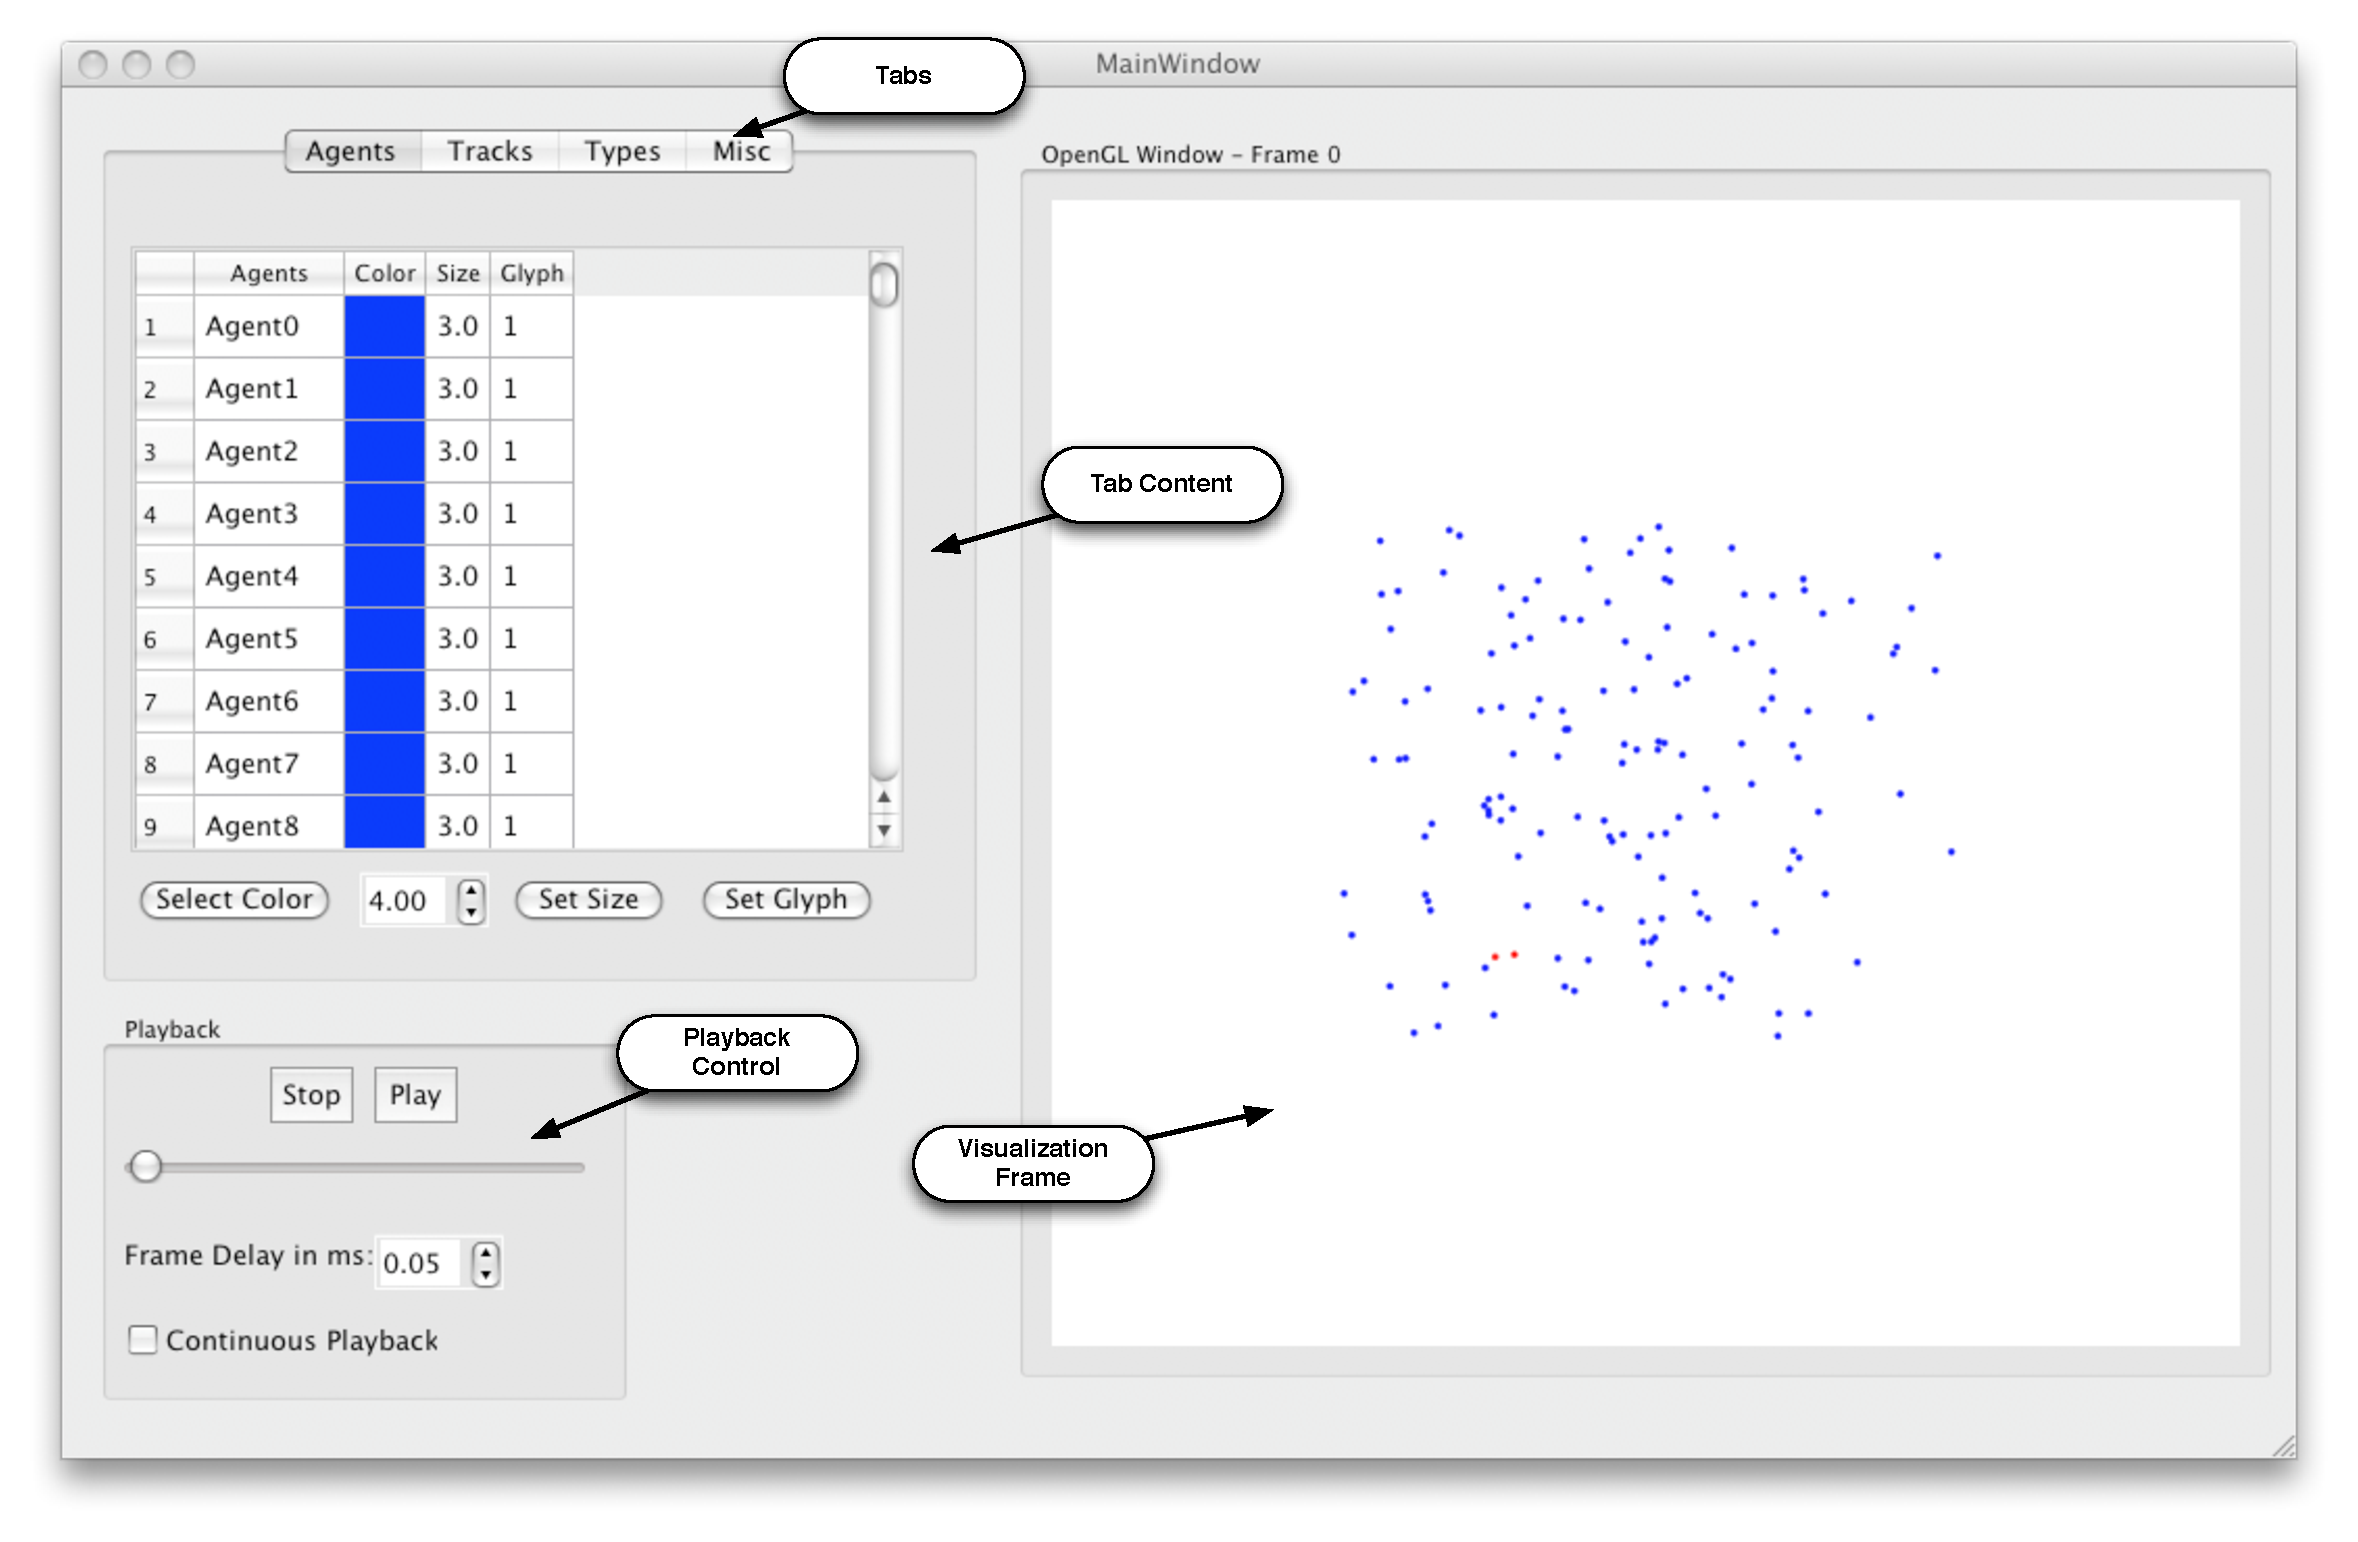
\includegraphics[scale=.45]{images/swarmvis-annotated.pdf}
\caption{The SwarmVis graphical user interface. 
here is only one window in our application and from it you can navigate to all commands and visualization options.
The interface is split between the user controls and the visualization itself. There are tabs at the top left that give
options for different visualizations in the tab content frame. The playback frame in the bottom left works similar to a
standard media player. The visualization frame shows the swarm with all selected visualizations applied to it. In this
screenshot, the user has two agents colored red with all other options standard. }
\label{AnnotatedWindow}
\end{figure*}

\section{Implementation}
SwarmVis is mostly  implemented in the C++ language and utilizes the Qt framework\cite{Qt:website}
to build the graphical user interface and to imbed an OpenGL window.
The user interface is split down the center,
the left side containing the majority of the user interface and the right side containing the graphical display.
The visualization frame in the right side can be rotated and zoomed by dragging and mouse-wheeling, respectively.
In general, we tried to keep the interface as simple and straightforward as possible.
A more detailed description of the user interface is given in Figure \ref{AnnotatedWindow}.
Changes made to the visualization through the interface happen in real-time, as the visualization is playing.
Lists and parameters are populated when a data set is loaded (more information about data sets is available in the appendix).

In the remainder of this section, we list the available visualizations in SwarmVis, what they convey, how they are implemented,
how they can be enabled, and how they can be modified.

\textbf{TODO: provide citations for where we got inspiration for each visualization.}


\subsection{Visualizations}





\begin{figure}
\centering
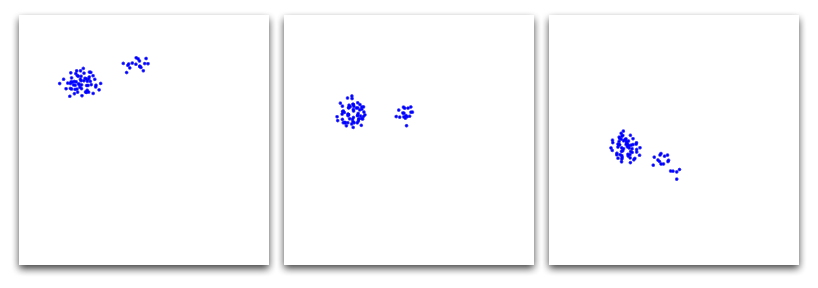
\includegraphics[scale=.282]{images/animation.png}
\caption{
Three captured frames from a swarm animation of three-dimensional flocking boids\cite{reynolds1987}.
When viewed in quick succession as frames in a video, the user
is able to detect the flocks' motion and structural changes.}
\label{Animation}
\end{figure}

\subsubsection{Animation}

The playback control (as seen in  seen in Figure \ref{AnnotatedWindow})
gives the user the ability to specify what is being shown in visualization frame.
The inspiration for this control is a standard media player with the ability to stop,
play and manually move through frames (with the slider).
In addition, the user can specify how fast the animation is created by adjusting the amount of delay between
frames (``frame delay" box).

Viewing a swarm over several time steps conveys a great deal amount of information. It conveys direction,
velocity and structure of the swarm by being able to see how it changes from time step to time step.
SwarmVis manages to be incredibly smooth even with a fast frame rate and hundreds of agents on a modern
computer\footnote{2.2 GHz MacBook Pro running Mac OS X 10.5}.
An example of this is shown in Figure \ref{Animation}, in which a swarm is shown to be
generally moving south with its sub-swarmsbeginning to merge.
All of our visualizations  that can be applied to the swarm (color, size, trails, tracks) can be seen in fluid animation.








\begin{figure}
\centering
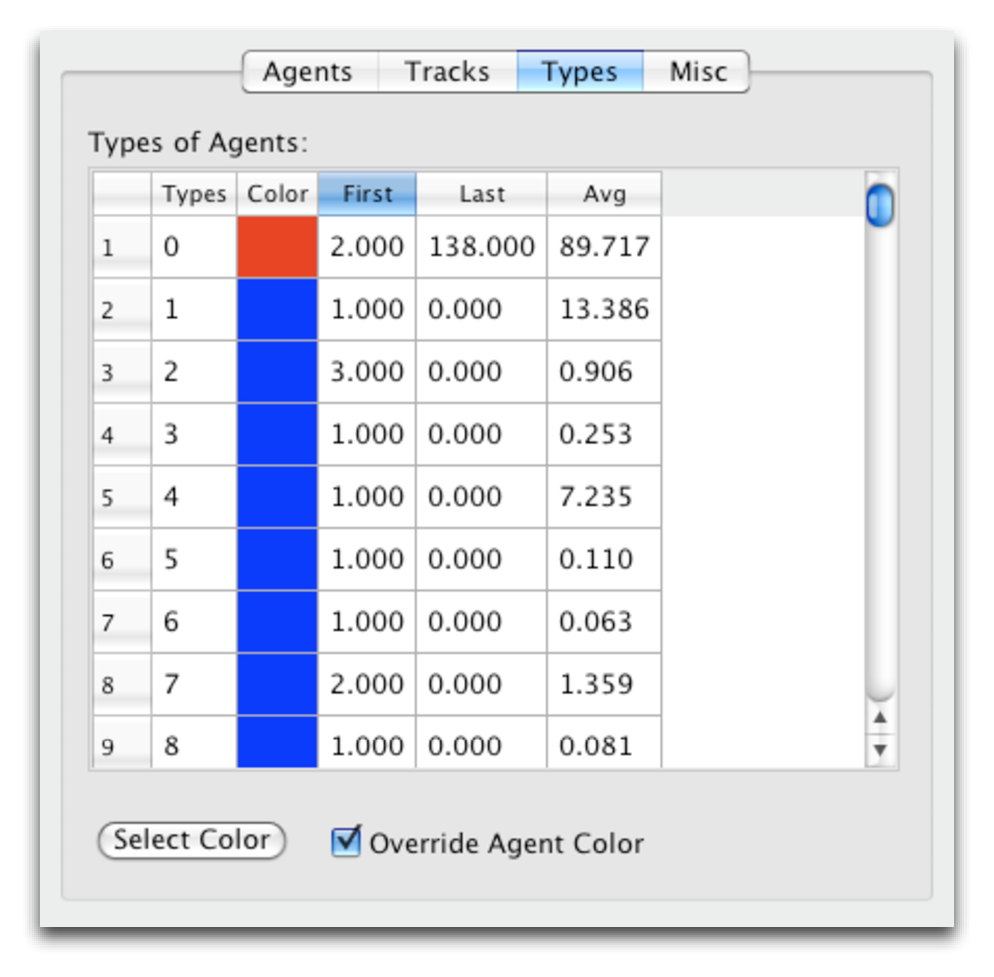
\includegraphics[scale=.5]{images/typestab.pdf}
\caption{
The Types tab shows the user which different subgroups exist in the swarm and allows the user to assign a specific
color to that group. Supplemental information helps the user
select the groups he wants: First (number of agents in that group in the first frame),
Last (number of agents in that group in the last frame), and Avg (average number of agents in that group during
the entire animation).}
\label{TypesTab}
\end{figure}

\begin{figure}
\centering
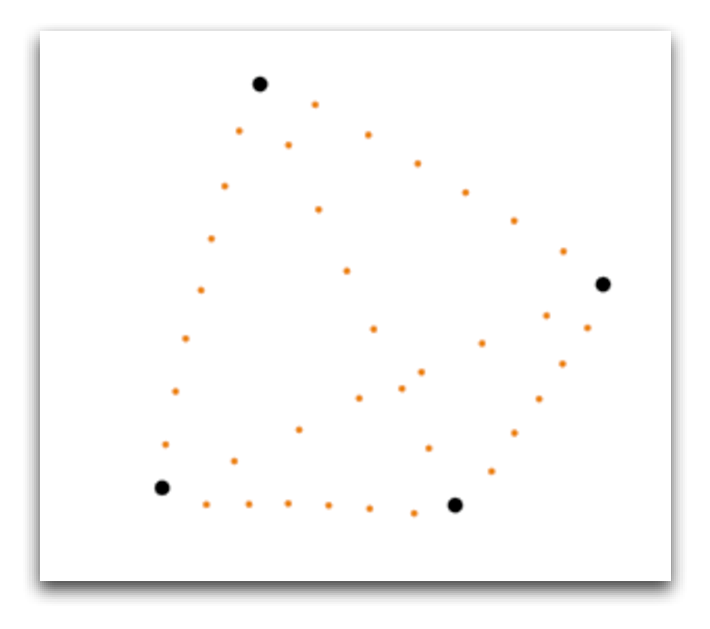
\includegraphics[scale=.7]{images/sizeandcolor.pdf}
\caption{
A captured frame from a swarm of tetrahedra-forming boids.
The corner agents have been given a larger size and a darker color than the edge agents.}
\label{SizeAndColor}
\end{figure}


\begin{figure}
\centering
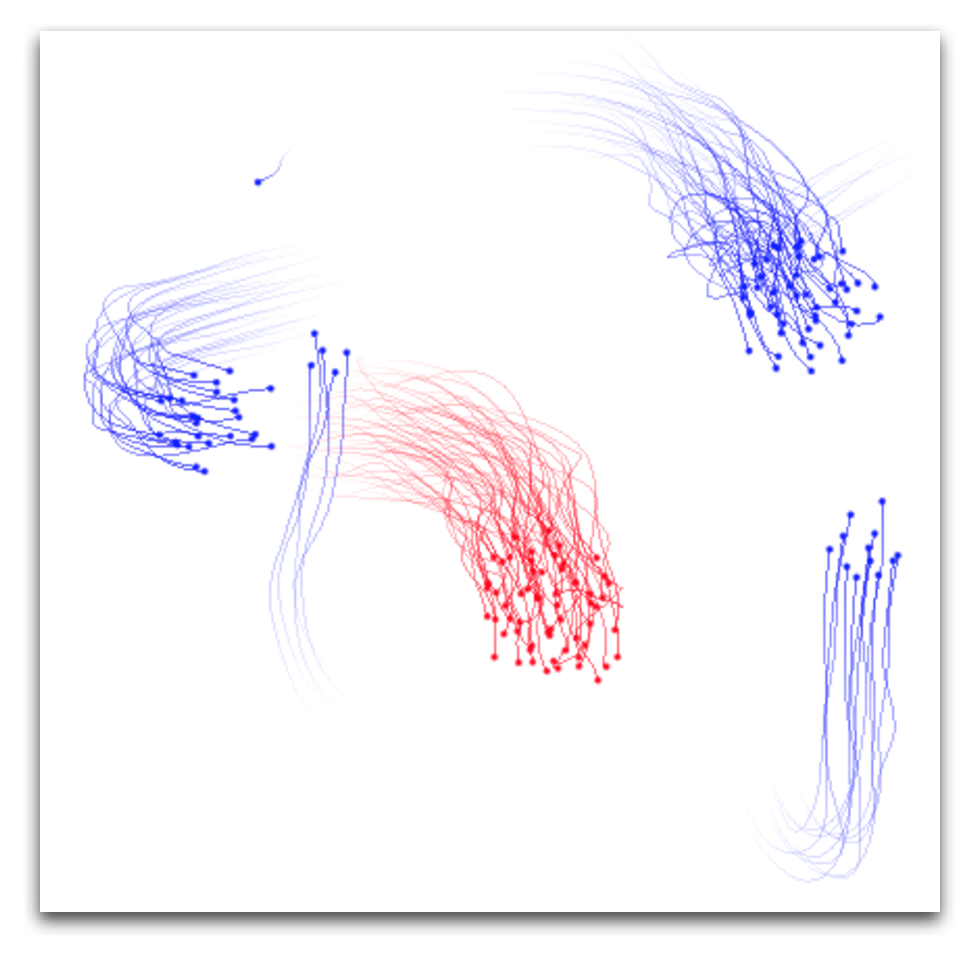
\includegraphics[scale=.5]{images/flockcolor.pdf}
\caption{
A captured frame from the three-dimensional flocking swarm shown in Figures \ref{ShowOff} and \ref{Animation}.
The trails in this image are of length 35 time steps and agents of a particular group are colored red.}
\label{FlockColor}
\end{figure}


\subsubsection{Color and Size}

An important feature of SwarmVis is the ability to track individual agents.
This can be done by selecting any number of agents of interest in the list of agents
(seen in the content frame of Figure \ref{AnnotatedWindow})
and changing their color or size with the button controls.
For example, the corner agents have been made bigger to emphasize their importance
in the tetrahedron swarm shown in Figure \ref{SizeAndColor}.

In addition, users can change
the color of all agents that are members of a specific group in the Types tab, as seen
in Figure \ref{TypesTab}. This feature can be used in addition to changing the size to
emphasize particular agents. For example, in the swarm shown in
Figure \ref{SizeAndColor}, we color the corners black and the edges orange. Another
example is shown in Figure \ref{FlockColor}, in which we colored the largest swarm
red and left the other swarms blue. Changing the color of the largest flock in the flocking domain is
particularly useful because it shows when two groups merge by changing the agents' colors
as they collide.
Also, this feature is great for creating figures for published articles in swarm research because
by changing the color and size, the writer can refer to specific agents as ``the bigger agents"
in the text instead of having to manually add labels to the images.





\begin{figure}
\centering
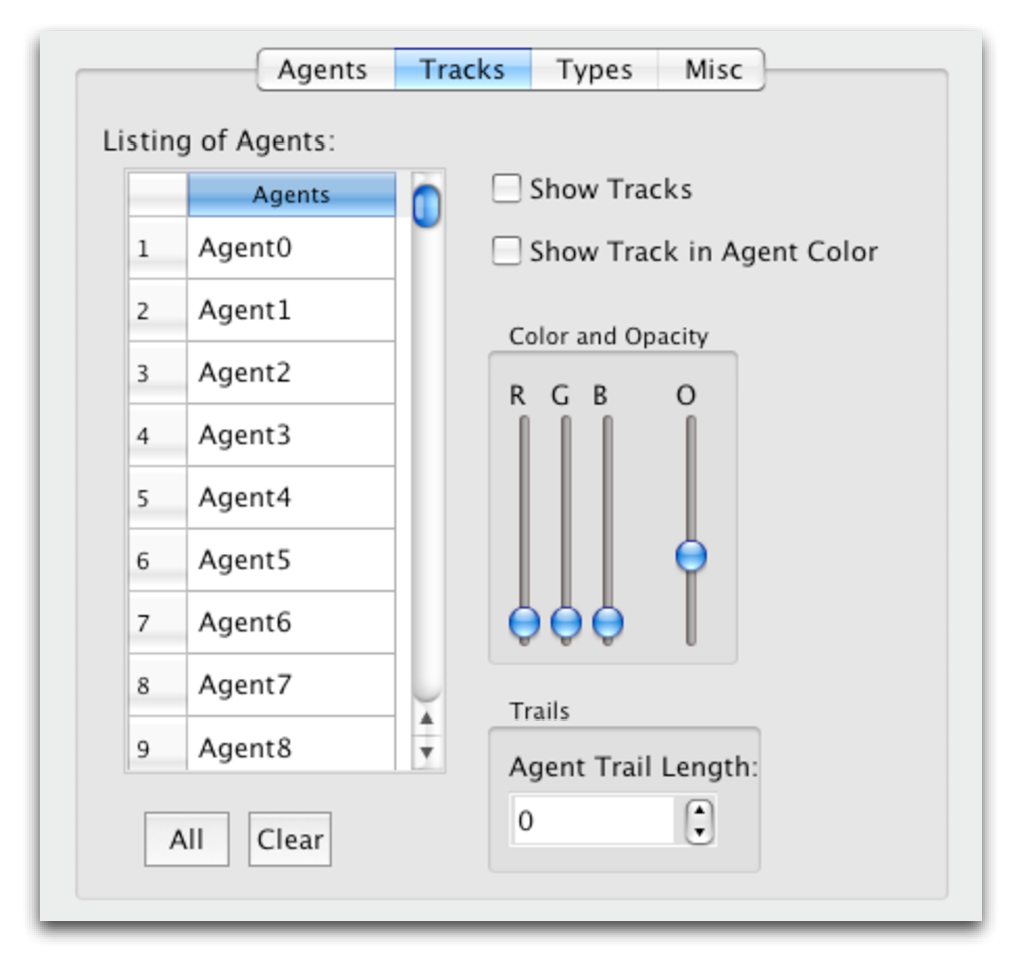
\includegraphics[scale=.5]{images/trackstab.pdf}
\caption{
The Tracks tab allows users to add tracks and trails to agents. The length of the trails can be adjusted 
with the ``Agent Trail Length" box. }
\label{TracksTab}
\end{figure}

\begin{figure}
\centering
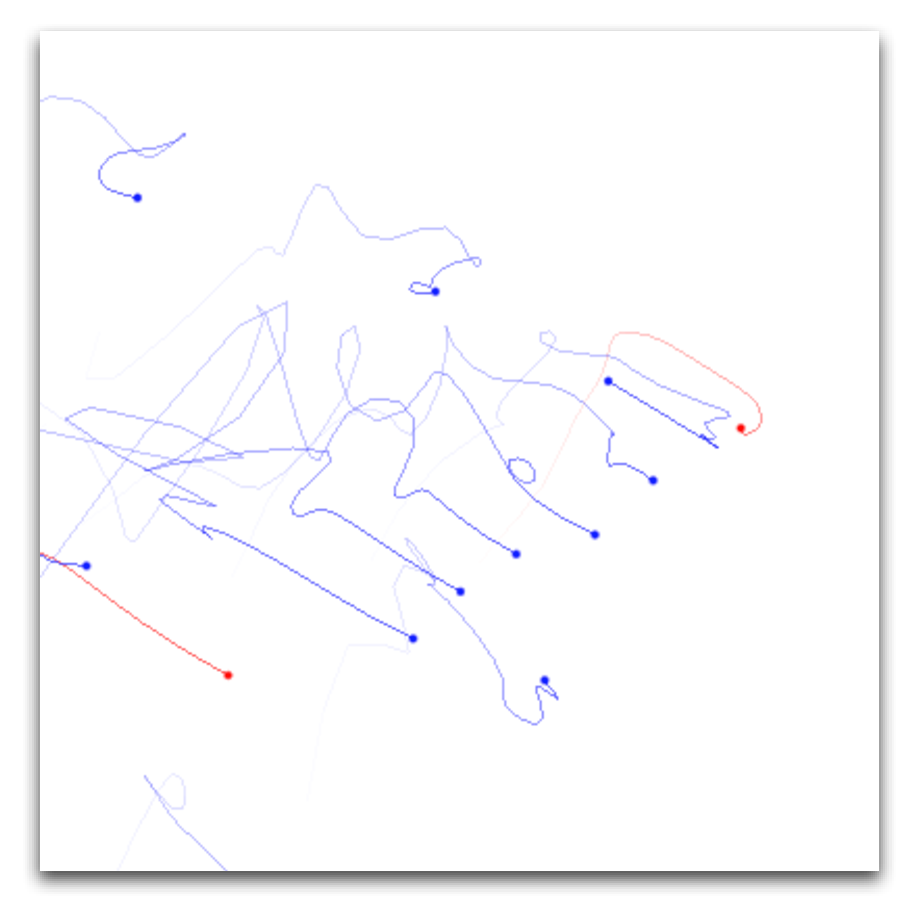
\includegraphics[scale=.5]{images/closeuptrails.pdf}
\caption{
A captured frame from a swarm of tetrahedra-forming boids shown in Figure \ref{SizeAndColor}.
Close up views of the swarm can convey much information about how agents interact with one another.
In this frame, we see how the rightmost red corner agent swapped places with the rightmost edge agent.
Then, edge agents fill in the gap by moving to the right. The different times in which each adjustment happened
is shown by how long ago a pattern happened in the trail.}
\label{CloseTrails}
\end{figure}

\subsubsection{Trails}

Trails are one of the most important features in SwarmVis because it conveys motion, previous positions, direction,
and change in structure, both in still images and videos. Trails are lines that hang behind agents, tracing
their previous positions. 
The trails are created by connecting previous positions of the agents with
successive lines that are more opaque near the current agent and less so further back in time.
The length of trails can be adjusted by modifying the number in the ``Agent Trail Length" text box, shown in
Figure \ref{TracksTab}.

Trails can be used to view swarm behavior at an abstract level, such as tracking the motion of several boid
flocks at once, as seen in Figures \ref{ShowOff} and \ref{FlockColor}.
One of the most powerful abilities of trails is to convey low-level behavior information in swarms. For example,
in Figure \ref{CloseTrails}, we can see that the rightmost corner agent (colored red) swapped position with the rightmost
edge agent (colored blue). Then, all the agents in that edge shifted down to accommodate.
The time delay in behavior is shown by the ``notch" in the path happened further ago for the left agents and more recently
in the right agents.
This visualization feature makes qualitative analysis of how the agents behave both at a low interaction level
and a high swarm emergent behavior level possible.







\begin{figure}
\centering
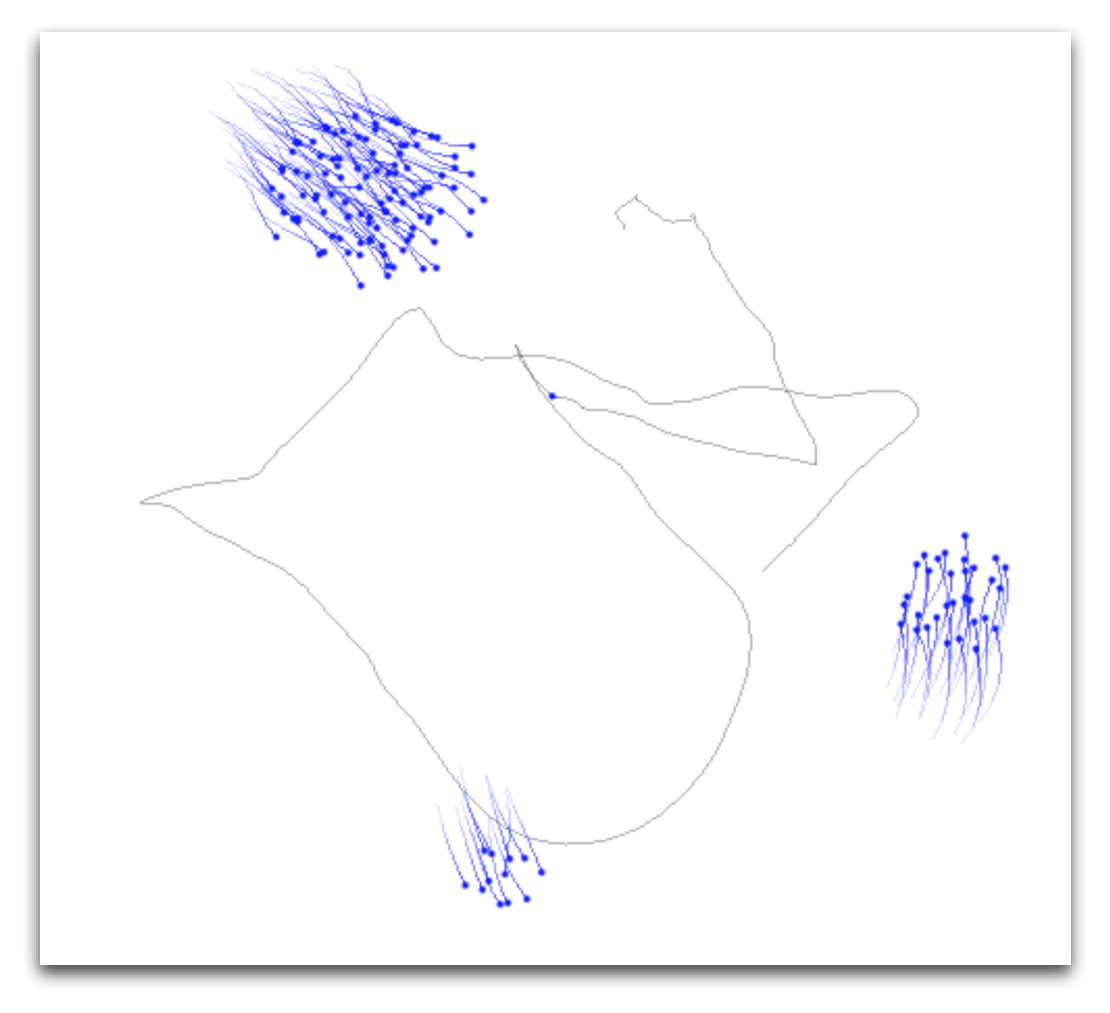
\includegraphics[scale=.451]{images/track.pdf}
\caption{
A captured frame from the three-dimensional tetrahedron Figures \ref{ShowOff}, \ref{Animation} and \ref{FlockColor}.
The lonely agent in the middle follows this gray path over its lifetime. The structure of the line in three-dimensional space
is seen much better when able to interactively rotate the view.}
\label{Track}
\end{figure}


\subsubsection{Tracks}

The Tracks feature is very similar to the trails feature
(they are implemented the same way), except that it shows the position of the agent over the entire
lifetime of the system. At any given frame, the agent will be somewhere on the track
For example, a track of a single agent is shown in Figure \ref{Track}.
Several agents can be selected at once in the list of agents in the Tracks Tab (Figure \ref{TracksTab}) to
have their trails all shown at once with the color specified by the ``Color and Opacity" sliders.
When tracks are used in conjunction with trails, the trails are overlaid on top of the tracks so that
both trail and track information is conveyed.

\section{Results}

To demonstrate the usefulness of SwarmVis, in this section we provide two walkthroughs as case studies, first,
a boid flocking domain and second, a tetrahedron-forming swarm.

\subsection{Case Study: Boid Flock}

\textbf{TODO: add content}

\subsection{Case Study: Tetrahedron-Forming Swarm}

\textbf{TODO: add content}

\section{Future Work}
SwarmVis is a complete application that has accomplished all the goals that we set out to achieve. 
However, there are a few user interface changes that would make usability better.
Also, we would like SwarmVis to visualize the instantaneous velocity and the depth of
agents since this information is not explicitly present in the
graphical display. These future improvements are discussed in this section.

In the future, we would like to make it easier to select agents and determine which agents are which in the graphical display.
To facilitate this, we hope to be able to show text labels that are adjacent to the agent in the visualization window.
These labels can show the name of the agent in the agent list.
Also, the ability to click agents in the visualization window will allow for greater interactivity and easier modification of agent-level colors and effects.

Currently, each visualization effect is controlled by a separate procedure.
Therefore, separate agent lists are kept in the Agents tab, the Tracks tab and the Types tab.
To make changes to an effect requires using that effect's tab and any changes made (e.g., color) are not reflected in the other lists.
Having an interactive global agent list that displays all necessary information will enable users to modify
the colors and effects on groups of agents more effectively. 

We also plan on adding the feature to change the representation of the agent itself to better display direction. Currently, direction is
inferred by the user by viewing the agents' trail, which may not be effective in every situation.
If agents were represented as three-dimensional arrowheads or perhaps other glyphs,
still images would convey very clearly the direction the agent is going on.

To further enhance the information conveyed in still images, we plan on determining a sufficient way to display depth.
We are not sure what the best technique for this would be, and no previous work to our knowledge has specifically dealt with this problem.

Finally, we plan on making SwarmVis extendable through a plug-in type framework. Any new visualization effects that are added
to SwarmVis must be hard coded into the source. This is not intuitive for a user that does not have knowledge of the source code
who wishes to add his own visualization to SwarmVis. Plug-ins could be simple programs that take the agent data as input and return
what the plug-in would like to have drawn on the screen. For example, the agent trails effect could be implemented as a plug-in, such
that it returns a list of lines to be drawn. A plug-in user interface will have to be implemented that allows users to manage plugins,
as well as use them. There should be some way for the plug-ins to interface with the global agent list to add informations to columns
and access information.


\bibliographystyle{IEEE}
\bibliography{cmsc636-swarmvis}

\appendix[User Guide]

\subsection{Compiling and Running}
SwarmVis was created to run on Unix-like systems, such as Mac OS X and GNU/Linux.
The following programs are required to compile SwarmVis:
\begin{itemize}
\item Qt 4.2
\item gcc/g++ 4.2.2
\item make
\end{itemize}
Note that some libraries from Qt4.2 may be needed to run SwarmVis in binary form.
We have tested SwarmVis on Mac OSX 10.5 and openSUSE Linux 11.

Run \texttt{qmake}, then run \texttt{make}, both in the root directory, to compile SwarmVis.
A binary will be created in the \texttt{bin/} directory. Execute this binary to run SwarmVis.

\subsection{Data File Format}
SwarmVis requires a specific file format for data sets that are to be loaded. The agents' position data is segmented into
separate files that each represent a single time step. These files are space-delimited data, with
each row representing an agent. For example, a swarm system with 100 agents depicted over 500 time steps
will have 500 files in a folder, each with 100 lines.

Each row entry in a file follows a format as well. The first two or three  columns (depending on dimensionality) are the
position data $(X, Y)$ or $(X, Y, Z)$, respectively. The last column is reserved for the group label, which may be used to pass
group membership data to SwarmVis.
For example, a well-formed line that conveys a three-dimensional
position with group information could be:
\begin{quote}
\texttt{10.15 5.24 84.85 CornerAgent}
\end{quote}
The listing of agents in each file should be stable. That is, the third line in one file and the third line in another file
should represent the same agent.

A plain-text information file containing important meta-data must accompany the frame files in the same directory.
The following variables must be defined (i.e., \texttt{VARNAME = VALUE}) in this file in order for the data to be loaded appropriately:
\begin{itemize}
\item \texttt{DIMENSIONS} (\texttt{2} or \texttt{3})
\item \texttt{AGENTS} (the number of agents)
\item \texttt{FRAMES} (the number frames/time steps)
\item \texttt{RANGEX} (the maximum X value)
\item \texttt{RANGEY} (the maximum Y value)
\item \texttt{RANGEZ} (the maximum Z value)
\item \texttt{AGENTTYPES} (\texttt{1} to track agent types, \texttt{0} if not)
\end{itemize}
At the bottom of this file, the keyword \texttt{FILES} must appear, followed by a list of frame files, in temporal order. The number
of files listed here must equal the number specified by the \texttt{FRAMES} variable. Also,
the number of lines in every file must match the number specified by the \texttt{AGENTS} variable. Below is a sample info file:
\begin{verbatim}
     DIMENSIONS = 3
     AGENTS = 150
     FRAMES = 446
     RANGEX = 600
     RANGEY = 600
     RANGEZ = 600
     AGENTTYPES = 1

     FILES
     frame000001.txt
     frame000002.txt
     ...
     frame000446.txt
\end{verbatim}

To load a data set in the SwarmVis application, navigate to ``Load Data" and select the info file.

\end{document}


